\documentclass[graphics]{beamer}
\usepackage{xcolor}
\usepackage{graphicx}
\usepackage{verbatim}
\usepackage{wrapfig}
\usepackage{tabularx}
\usepackage{multirow}
\usepackage{amssymb}
\usepackage{pifont}
\usepackage{tikz}
\def\Checkmark{\tikz\fill[scale=0.2](0,.35) -- (.25,0) -- (1,.7) -- (.25,.15) -- cycle;} 

\useoutertheme{shadow}
%\usecolortheme{orchid}
\usecolortheme{seahorse}
\newcommand{\cmark}{\text{\ding{51}}}
%\newcommand*{\GtrSim}{\smallrel\gtrsim}

% math commands
\newcommand{\be}{\begin{eqnarray}}
\newcommand{\ee}{\end{eqnarray}}
\newcommand{\beq}{\begin{equation}}
\newcommand{\eeq}{\end{equation}}
\def\simless{\mathbin{\lower 3pt\hbox
      {$\rlap{\raise 5pt\hbox{$\char'074$}}\mathchar"7218$}}}
\def\simgreat{\mathbin{\lower 3pt\hbox
      {$\rlap{\raise 5pt\hbox{$\char'076$}}\mathchar"7218$}}} %> or of order

% variables

\def\toonscale{0.45}
\def\mboxy#1{\mbox{\small #1}}

\defbeamertemplate*{title page}{customized}[1][]
{
  \usebeamerfont{title}\inserttitle\par
  \usebeamerfont{subtitle}\usebeamercolor[fg]{subtitle}\insertsubtitle\par
  \bigskip
  \usebeamerfont{author}\insertauthor\par
  \usebeamerfont{institute}\insertinstitute\par
  \usebeamerfont{date}\insertdate\par
  \usebeamercolor[fg]{titlegraphic}\inserttitlegraphic
}
\begin{comment}
\AtBeginSection[]{
  \frame{
    \frametitle{Outline}
    \tableofcontents[currentsection]
  }
}
\end{comment}


\title{\textcolor{red}{Cosmic Coherence}}
%\subtitle{}
\author[U. Pen]{{
{ 
\textcolor{green}{\small R. Main, D. Simard, D. Baker, F. Lin,
  A. Roman, A. Patil, 
F. Kirsten, I. Yang, V. Marthi}
}, 
\textcolor{red}{\small M. van Kerkwijk, K. Vanderlinde, JP Macquart,
  U. Pen} 
\textcolor{while}{\small and more scintillometers}
}
\\[8mm] 
}
\date{\textcolor{blue}{October 5, 2020}}


\begin{document}


%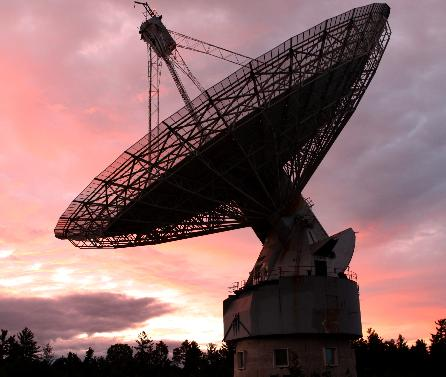
\includegraphics[width=4.4in]{Figures/IMG-7749-ARO-crop.JPG}

\frame{
\vspace{-0.5in}
\begin{center}  
%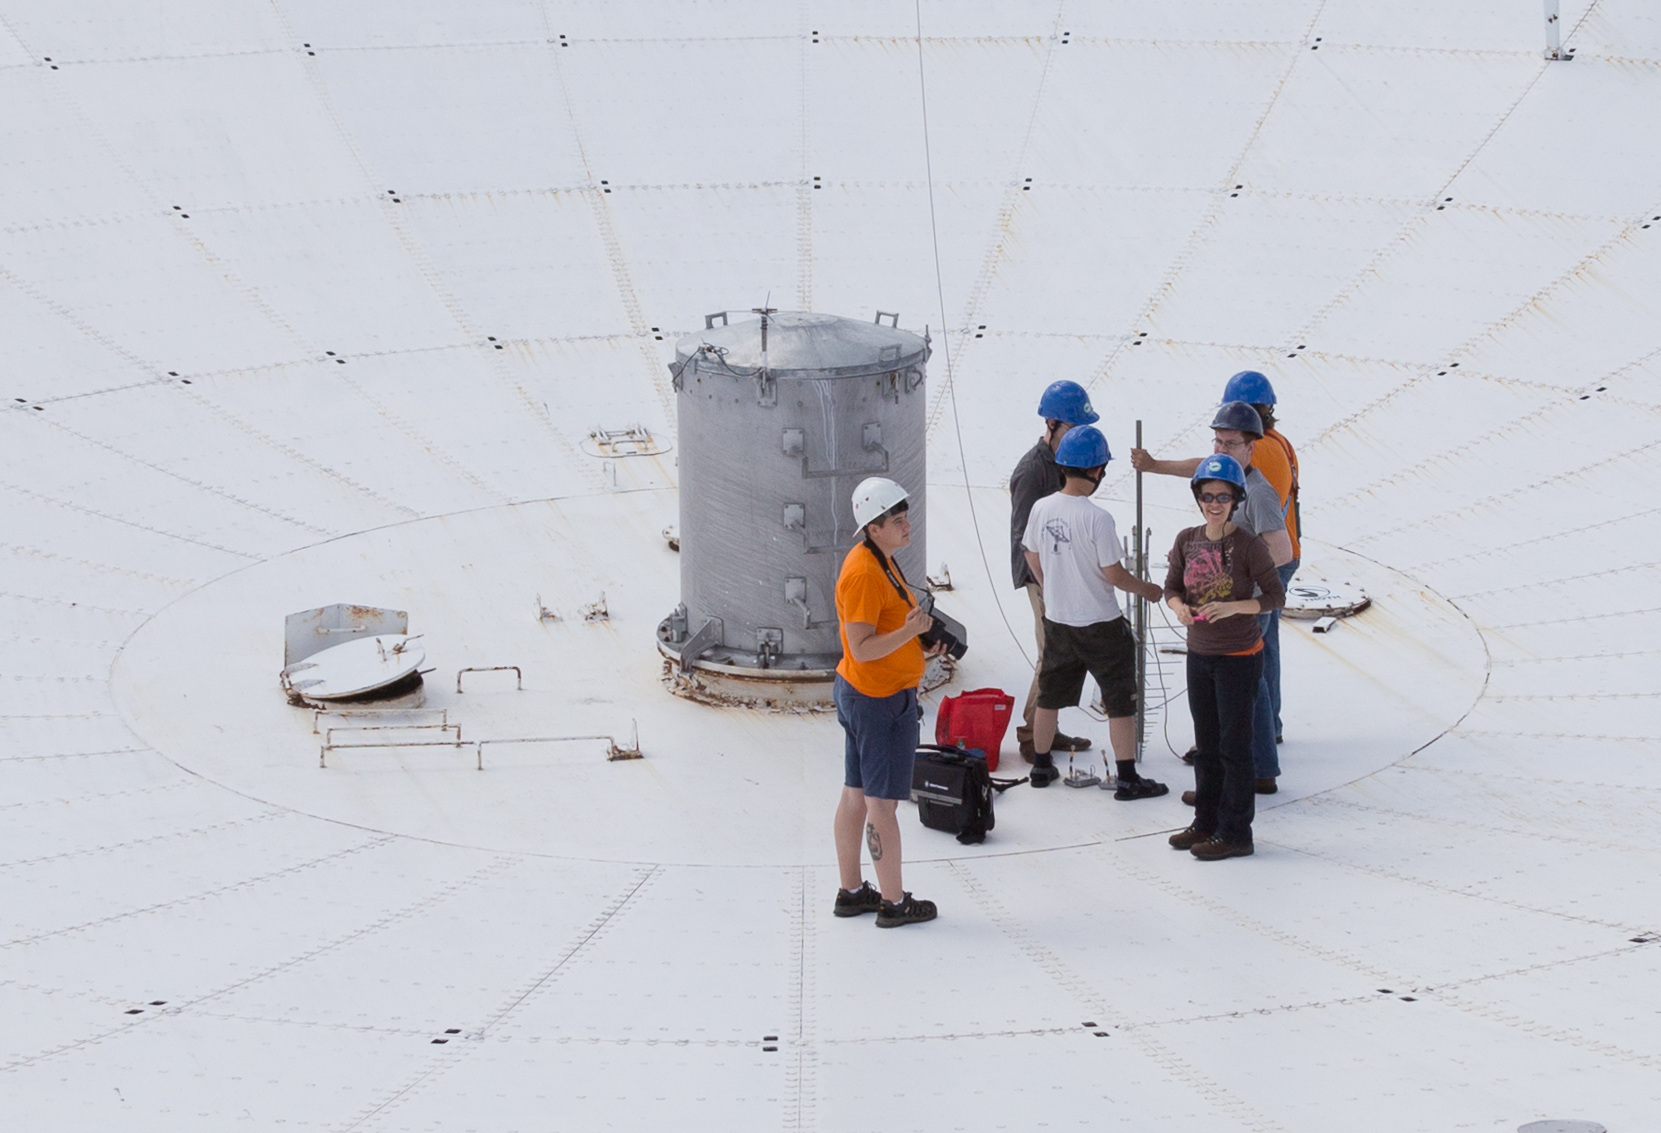
\includegraphics[width=4.4in]{Figures/IMG-0438-by-Andre-cropped.jpg}
\end{center}
\begin{picture}(320,250)
\put(-50,60){
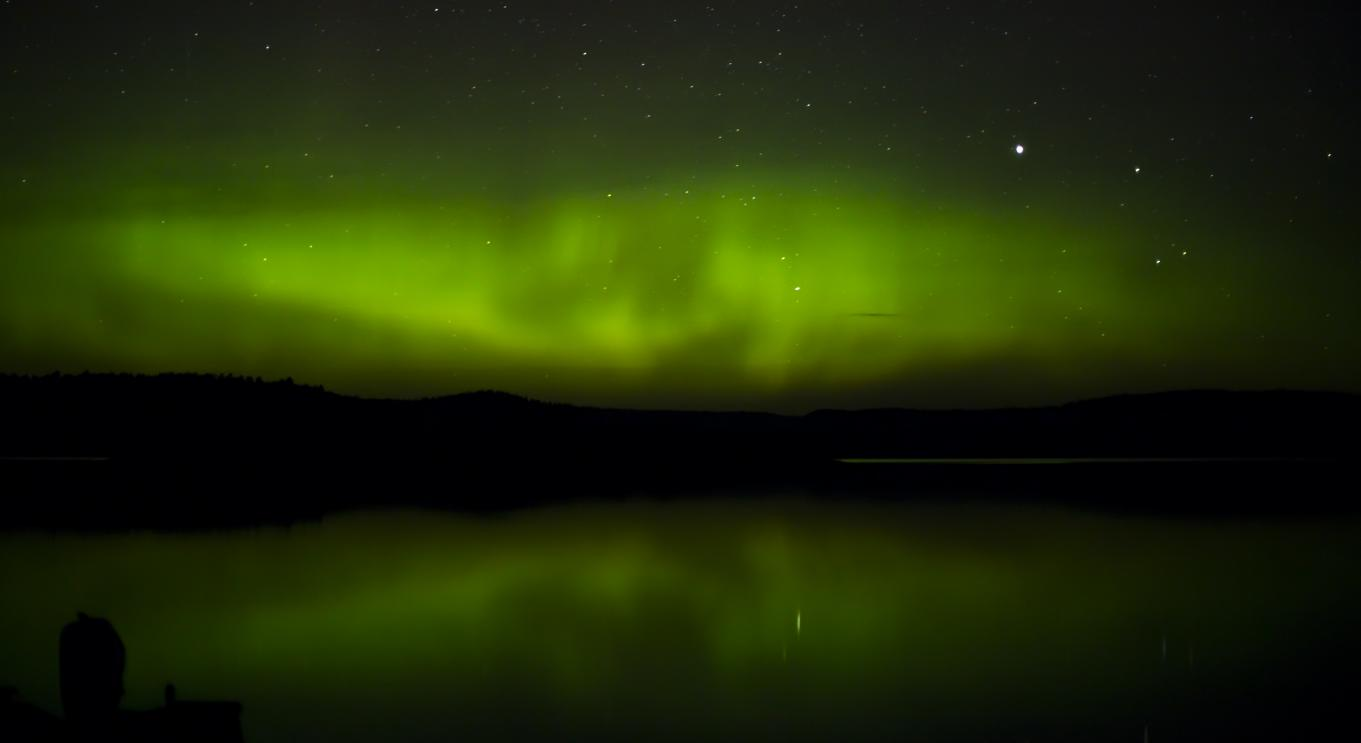
\includegraphics[width=5.5in]{Figures/traverse-aurora.jpg}}
\end{picture}
\vspace{-4in}
\\
image credit: Andre Recnik
\\
\vspace{1in}
%\titlepage
}


%\section*{Introduction}
\section{Introduction}

\begin{comment}
  \subsection{Outline}

  \frame{
    \frametitle{Outline}
    \tableofcontents
  }
\end{comment}

  \frame{
    \frametitle{Cosmic Coherence}
    \begin{itemize}
      \item cosmological coherence: traditional info from power
        spectrum, little use of phase information
      \item probed by galaxy spin directions (Yu, ULP, Wang 19),
        helicity (Motoch, Yu, Pen 20)
      \item phase coherence provides unique precision probes: e.g. LIGO
      \item FRB and pulsar radiation maintains phase coherence in the
        radio band, resulting in interference phenomena (Jow, Foreman,
        ULP 20, Feldbrugge Turok ULP 20)
      \item allows coherent VLBI measurements on earth  (Baker++
        20 in prep)
      \item potential tests of GR, GW, DE, DM, pulsar emission, EoS, 
      \item initial results on FRBs, pulsar emission, scalar gravity
        (Masui++ 16, ULP+14)
      \item open new opportunity for space VLBI
    \end{itemize}
    \vspace{-.01in}\hspace{2in}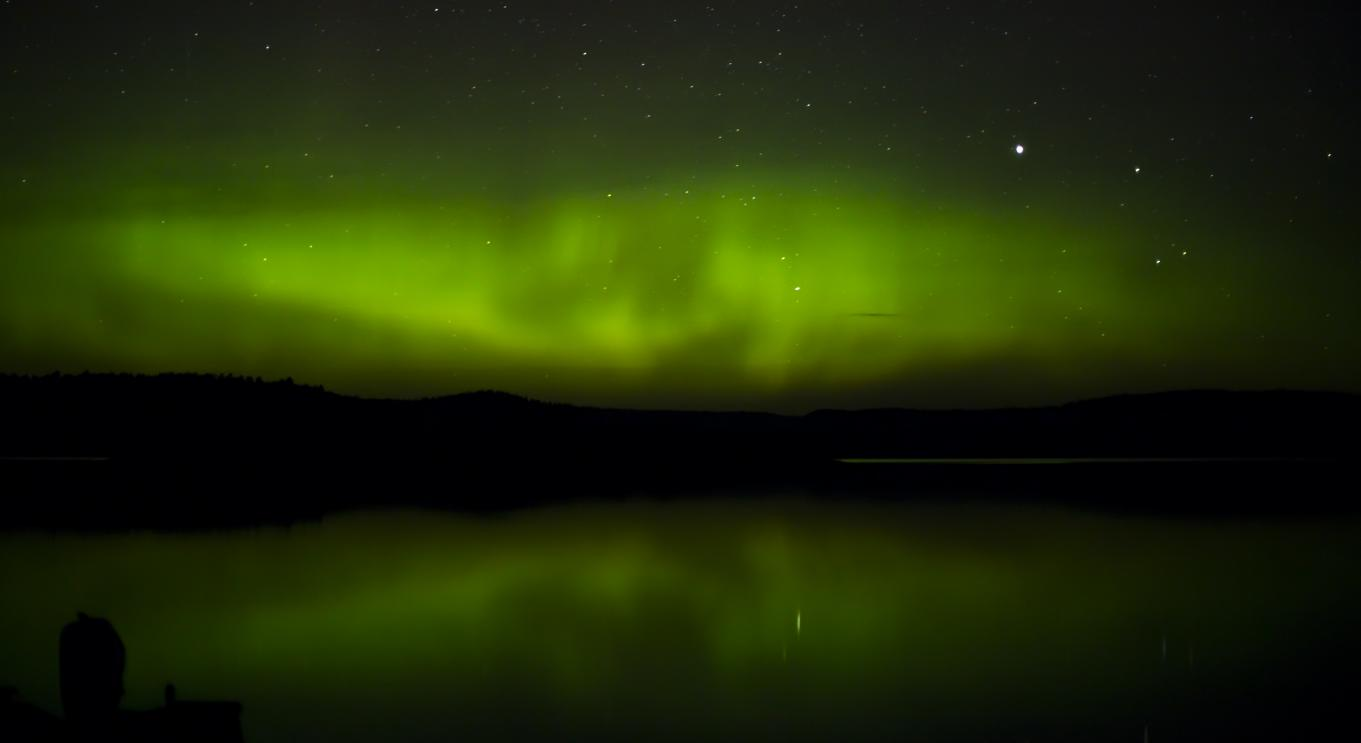
\includegraphics[width=0.3\textwidth]{Figures/traverse-aurora.jpg}
  }



\end{document}
